\documentclass[10pt]{article}
\usepackage[margin=0.8in]{geometry}
\usepackage{graphicx,hyperref,helvet}
\renewcommand{\familydefault}{\sfdefault}
\renewcommand{\ttdefault}{phv}
\pdfcompresslevel=9
\pdfobjcompresslevel=3
\hypersetup{colorlinks=true,urlcolor=blue}
\setlength{\parskip}{6pt}
\setlength{\parindent}{0pt}
\begin{document}
\begin{center}
{\Large Cubic-extension transfer: frozen evidence import}\\[5pt]
2026-10-25\quad Study: \texttt{cubic\_extension\_transfer\_20261025}
\end{center}

\textbf{Status.} Historical SageMath 10.6 source and recorded certificates;
no new research experiment, native performance result, or leaderboard promotion.

\textbf{Question.} When can a prime-order elliptic-curve logarithm over a cubic
extension be transferred into a usable plane-quartic Jacobian over the base
field, and what obstructs the twelve-candidate construction?

\textbf{Recorded finite result.} The retained example over the cubic extension
of the field with 157 elements has source prime order 3868159. All twelve
transverse targets have independently certified order 3871629. Two
nonprepared sources each have a unique rational degree-three isogeny into
that all-obstructed prepared model. A second step gives a usable target, and
the retained complete solver recovers scalar 271828 on the original curve.
This is a counterexample to a total-one-step guarantee within the specified
construction. One extra step after torsion preparation remains open.

\textbf{Structure.} The recorded 109-field comparison has different coverage
at the same geometric endomorphism discriminant, -21195. The complete finite
CM screen contains twelve Frobenius orbits and one all-obstructed orbit. A
degree-five isogeny repairs it while preserving the three-torsion type and
endomorphism order. These statements have the source report's ordinary,
non-subfield, prime-order and transverse-kernel hypotheses.

\begin{center}
\fbox{Source points}\quad\textgreater\quad
\fbox{Prepared model}\quad\textgreater\quad
\fbox{Usable quartic}\\[8pt]
\fbox{Actual divisor images}\quad\textgreater\quad
\fbox{Target logarithm}\quad\textgreater\quad
\fbox{Source verification}
\end{center}

\textbf{Recorded checks.} Ten complete prototype transfer cases and seven
targeted exceptional-input checks are retained. The saved verifier checks
source scalars, exact line intersections, large-prime graph substitutions
and modular systems. It is not a cross-host or independent-agent native audit.

\textbf{Timing limits.} The frozen records used Sage and a simple source rho
control; some jobs ran concurrently. They do not supply isolated native
operation counts, the strongest folded rho, an ecbench audit, or external-tool
qualification. The historical seconds are diagnostics; no cost ranking,
new exponent, fastest-tool status or deployed-curve conclusion is admitted.

\textbf{Publication.} The source bundle contains 164 original files. This PR
includes 159 byte-for-byte files and hash manifests for five original files
awaiting unchanged S3 upload and readback. No remote availability is claimed.
Conductor, Cargo/Rust and Lean/Lake are unavailable locally. Repository-wide
release tests, native replay, faithful Lean bridges and full artifact
hydration remain open. See \texttt{PUBLICATION.json} and the admission problem.

\textbf{Source links.} Relative to the study directory:
\begin{itemize}
\item \path{historical/extension-field-experiments/research_lead/FOUR_TRACK_RESULTS.md}
\item \path{results/forced_two_step_audit.json}\\
\path{results/explicit_forced_two_step_witnesses.json} under that research lead.
\item \path{results/forced_source_pipeline.json},
\path{results/endomorphism_audit.json}, and \path{results/cm_coverage.json}.
\end{itemize}

\newpage
\begin{center}
{\large Frozen prepared-component figure}\\[8pt]
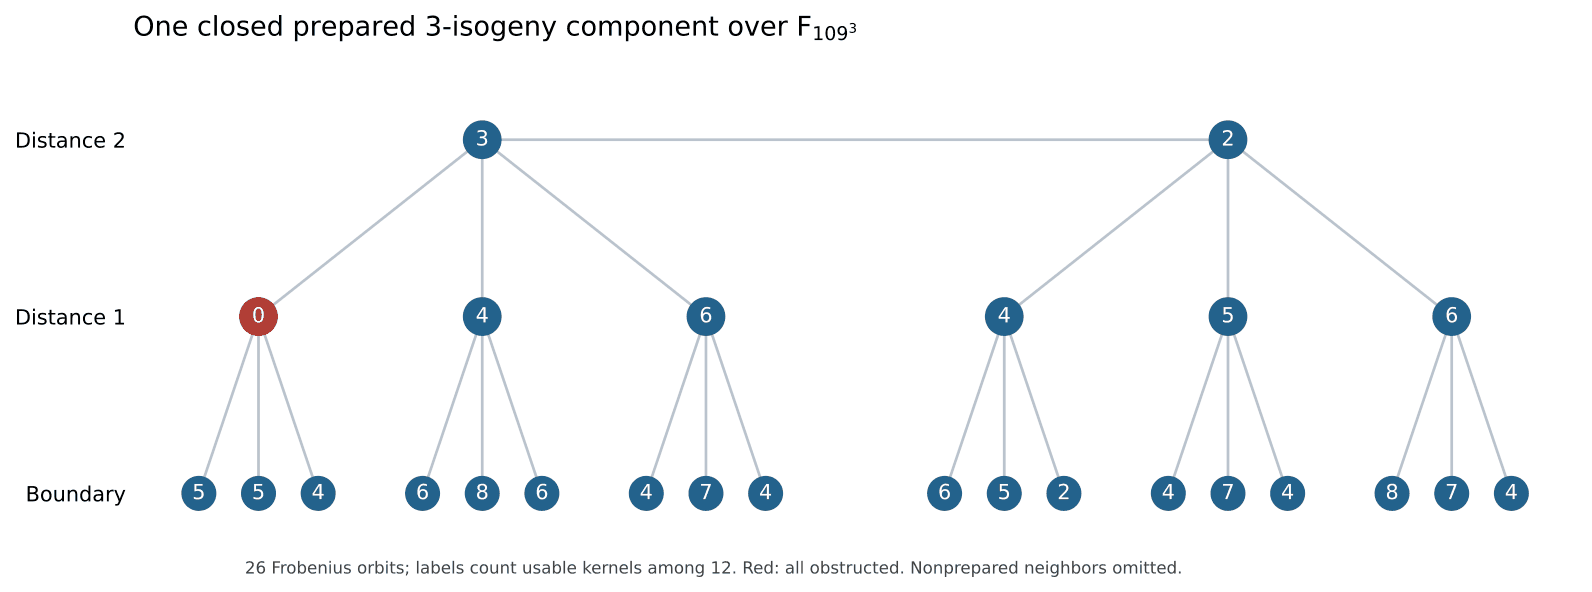
\includegraphics[width=\textwidth]{component-150.png}
\end{center}

This is the original study's component figure, rendered from its frozen SVG.
It records 26 prepared Frobenius orbits over the cubic extension of the
109-element field. Labels count usable kernels among twelve; red marks zero
coverage. Nonprepared neighbors are omitted. The exact models and edges are
in \path{results/neighborhood_component.json}; the source and proof scope
are in \texttt{FOUR\_TRACK\_METHOD.md}. This is a historical figure, not a new
repository-standard volcano-renderer run or a geometric formalization.

The canonical scoreboard, registry, benchmark index and IC leaderboard are
unchanged because the historical diagnostics have not met their admission
gates. A later native study must freeze its inputs, isolate and fully price
both arms, use the strongest applicable reference, independently replay the
answers and satisfy the validation schema before a promotion.

\textbf{Original bundle SHA-256:}\\
\texttt{6c6e079c8ebb64b52f03039bad743dc0948d0f1953b9f528b76e684959405aba}
\end{document}
